\section{Antennen und Ausbreitung \formelbuch{131}}
\subsection{Luftkanal \formelbuch{133}}
\begin{tabular}{ll}
\parbox{8cm}{
    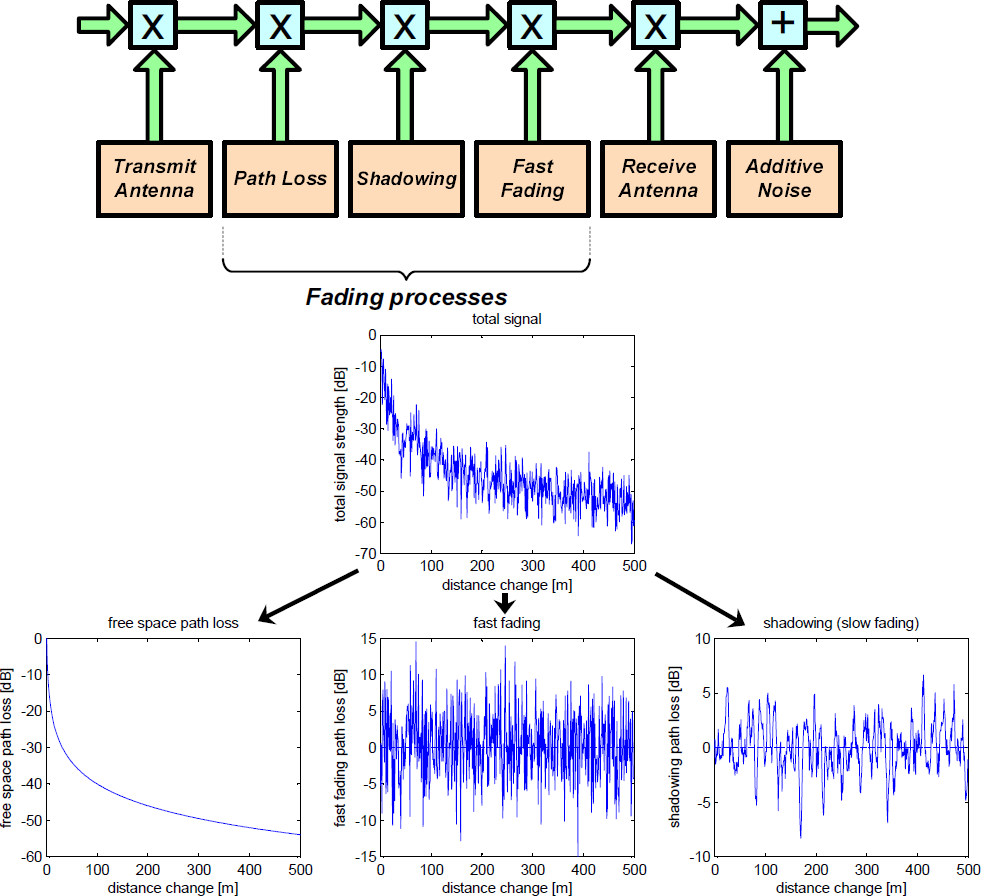
\includegraphics[width=7cm]{./bilder/antennas-noisetypes.png}}
    
& \parbox{10cm}{
    Rauschtypen:
    \begin{liste}
        \item Additives Rauschen
        \begin{liste}
            \item Thermisches, Flicker/Funkel/$\frac{1}{f}$, Shot Rauschen
            \item Atmosphärischer Einfluss, Kosmische Strahlung, Störungen von
            anderen el. Quellen
        \end{liste}
        \item Multiplikatives Rauschen
        \begin{liste}
            \item Richtungsabhängigkeit der Antennen
            \item Reflektionen
            \item Absorptionen
            \item Streuungen (Scattering)
            \item Beugung (Diffraction)
            \item Brechnung (Refraction)
        \end{liste}
    \end{liste}}
\end{tabular}

\subsection{Einführung \formelbuch{135}}
\begin{liste}
    \item Pfadverlust in Kabel: Linear zur Distanz; in der Luft: Logarithmisch zur Distanz
    \item Nah- \& Fernfeld: Grenze bei $R = \frac{2L^2}{\lambda}$
    \item Impedanz in der Luft: 
    $Z=\frac{|E|}{|H|}=\sqrt{\frac{\mu_0}{\varepsilon_0}}=120\pi \,\Omega= 377\,\Omega$
\end{liste}


\subsection{Antennen-Charakterisierung \formelbuch{140}}
\begin{tabular}{ll}
\parbox{6cm}{
    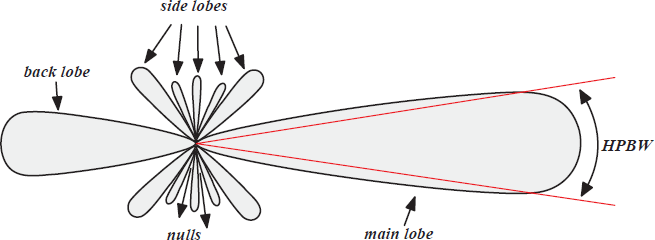
\includegraphics[width=6cm]{./bilder/antennas-radiation-pattern.png}}
& \parbox{12cm}{
\begin{liste}
	    \item Reziprozität: Charakteristiken der Antennen bleiben gleich, egal ob Antenne
	    als Sender oder Empfänger gebraucht wird.
	    \item Radiation Pattern (Richtcharakteristik): 
	    \begin{liste}
		    \item {\em Half-power beamwidth} (kurz {\em beamwidth} oder HPBW): Winkel
		    zwischen beiden half-power Punkten in der main lobe.
		    \item {\em Front-back ratio}: Verhältnis zwischen Peak Amplituden der main
		    und back lobe.
		    \item {\em Sidelobe level}: Verhältnis der grösste Amplitude der side
		    lobe und dem peak der main lobe.
	    \end{liste}
	\end{liste}
	}
\end{tabular}\\
\begin{liste}
    \item Antennenfläche (keine physikalische Interpretation): 
        $P = AS; \qquad A = \frac{\lambda^2 G}{4\pi} \quad G_{\text{dB}} = 10
        \log\left(\frac{4A\pi}{\lambda^2}\right)$
    \item Effektive Antennenlänge: 
    $V= E \frac{l_{\text{eff}}}2 = \sqrt{\frac{|E|^2AR}{120\pi \Omega}}$
    $;\qquad$ $l_{\text{eff}} = \sqrt{\frac{AR}{30\pi \Omega}}$
    \item Antennenfaktor: $k = \frac{E}{V} = 20 \log
    f_{\text{MHz}}-29.78-G_{\text{dBi}}$
    \item Polarisation: Vertikal, horizontal; Recht-Hand (RHCP)/
    Link-Hand Zirkular (LHCP): Definition schwierig \formelbuch{147}
    \item Antenneneffizienz: $\eta = \frac{R_{\text{rad}}}{R_{\text{rad}} +
    R_{\text{loss}}}$
    \item Antennnegewinn (Gain): $G=\eta \cdot D$ ($D$ = maximale Direktivität)
    \item Bandbreite: Bereich, wo $G < 3dB$ bzw. VSWR $< 2:1$
    \item Einheiten: $\underbrace{0dBd}_{\text{\tiny{G von $\lambda/2$-Dipol}}}
    = \underbrace{2.15dBi}_{\text{\tiny{G von isotropischer Antenne}}}$
\end{liste}

\subsection{Antennentypen \formelbuch{148}}
\subsubsection{Übersicht \formelbuch{153}}
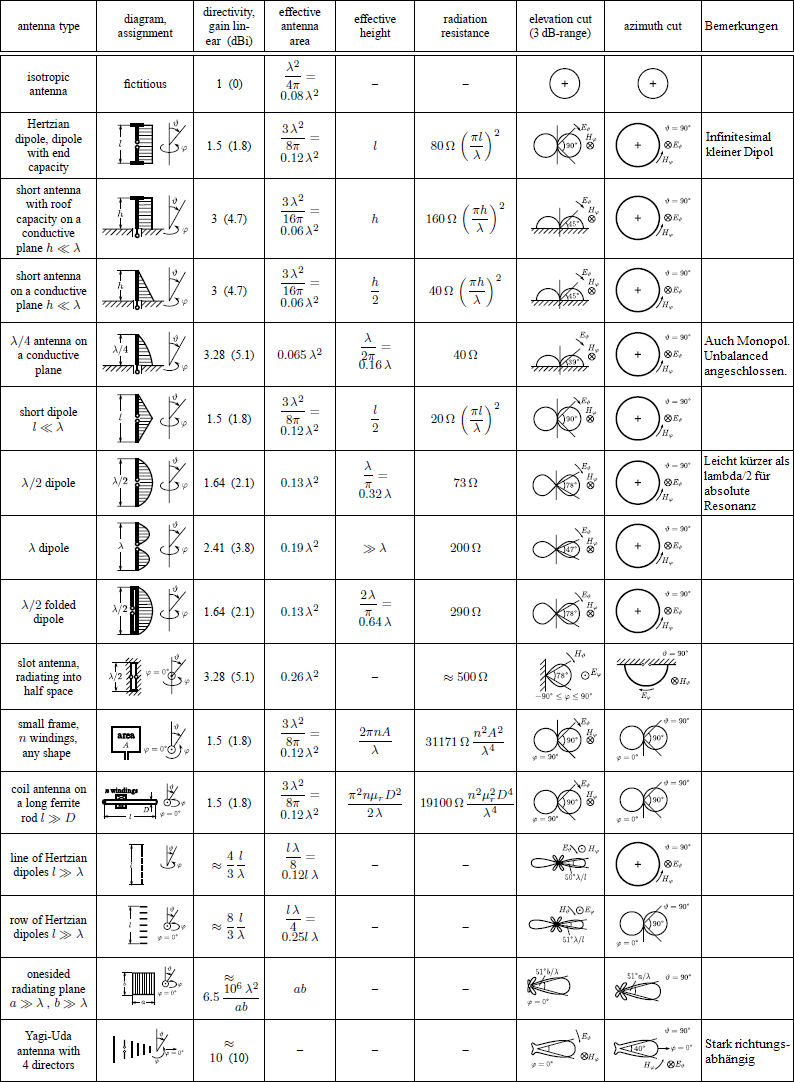
\includegraphics[angle=90,width=19cm]{./bilder/antennas-overview.png}

%\subsubsection{Weitere Antennentypen \formelbuch{150}}
%\begin{tabular}{ll}
%\parbox{11cm}{
%    \textbf{Logarithmisch Periodische Antenne (LogPer):} \\
%    Ähnlich wie
%    Yagi-Antenne, aber ausgerichtet auf hohe Bandbreite .\\
%    
%    
%    \textbf{Loop-Antenne:} \\
%    Ineffizient, dafür kleiner Platzverbrauch.
%    Herstellung als viereckige Metallstreifenloops oder als PCB.\\
%    
%    
%    \textbf{Patch- bzw. Microstrip-Antenne (rechts):}\\
%    V.a. in GPS und mobilen Geräten benutzt. Quadratischer oder runder Patch
%    über Groundplane. $W = \lambda/2 \qquad L \approx 0.49
%    \frac{\lambda}{\sqrt{\epsilon_r}}$ 
%    }
%& \parbox{8cm}{
%    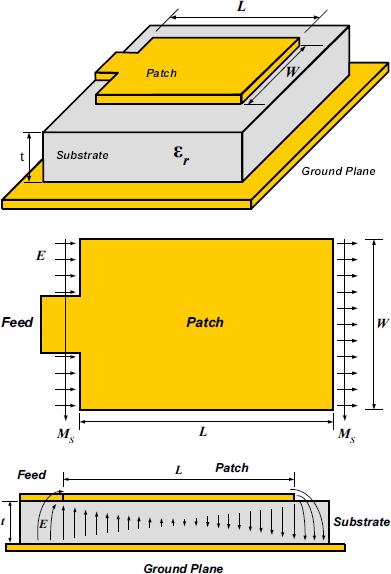
\includegraphics[width=5cm]{./bilder/antennas-patch.png}
%    }
%\end{tabular}

%\subsection{Antennenmessungen \formelbuch{154}}
\newpage

\subsection{Luftlose Übertragung \formelbuch{155}}
\begin{tabular}{|l|c|}
\hline
\textbf{Modell}
    & \textbf{Abbildung}\\
\hline
\hline
\parbox{10cm}{
    \textbf{Free-space propagation \formelbuch{155}} \\
    \begin{minipage}{6cm}
	    \begin{liste}
	        \item Keine Reflektionen
	        \item Keine Hindernisse
	        \item Kein Multipath
	        \item Zu optimistisch/idealisiert
	    \end{liste}        
    \end{minipage}
    \begin{minipage}{3cm}
        $$ P_R= \frac{P_TG_T}{4\pi r^2} A_R $$
        $$ \frac{P_R}{P_T} = G_TG_R \left(\frac{\lambda}{4\pi r}\right)^2  $$
    \end{minipage}

    $$L=\frac{P_TG_TG_R}{P_R} = \left(\frac{4\pi r}{\lambda}\right)^2 =
    \left(\frac{4\pi rf}{c}\right)^2$$ 
    $$L\,\text{[dB]} = -147.6 + 20\log r + 20\log f$$ }
    & \parbox{3cm}{
        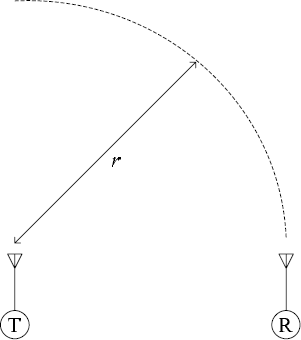
\includegraphics[width=3cm]{./bilder/propagation-freespace.png}
        } \\
\hline
\parbox{10cm}{
    \textbf{Open-field/Plane-earth propagation \formelbuch{156}} \\
    \begin{liste}
        \item Keine Hindernisse    
        \item Einfache Reflektion am Boden (zwei Pfade)
        \item Zweiter Pfad kann konstruktiv oder destruktiv sein
    \end{liste}
    $$L= 4\frac{\pi r}{\lambda}^2
       \sin^{-2} \frac{2\pi h_bh_m}{\lambda r} \quad \text{für } r <
       r_x=\frac{4h_bh_m}{\lambda}$$ 
    $$L= \frac{r^4}{h_b^2h_m^2} \quad \text{für } r > r_x$$
    }
    & \parbox{5cm}{
        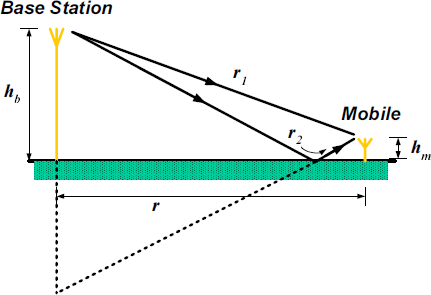
\includegraphics[width=5cm]{./bilder/propagation-openfield.png}
        } \\
\hline
\parbox{10cm}{
    \textbf{Simulation (rechts) \formelbuch{158}}:\\
    $h_b=20\,$m, $h_m=1.5\,$m, $f=1\,$GHz \\
    
    \textbf{Weitere Modelle}\\
    Exponent $n$ der Entfernung $r^n$ hauptsächlich massgebend für Modell.
    Weitere Möglichkeiten:
    
    \begin{tabular}{|l|r|}
	\hline
	environment & path-loss exponent $n$      \\ \hline \hline
	free space                     & 2        \\ \hline
	open field (long distance)     & 4        \\ \hline
	cellular radio, urban area     & 2.7--4   \\ \hline
	shadowed urban cellular radio  & 5--6     \\ \hline
	in building, line-of-sight     & 1.6--1.8 \\ \hline
	in building, obstructed        & 4--6     \\ \hline
	\end{tabular}
    }
    & \parbox{8cm}{
    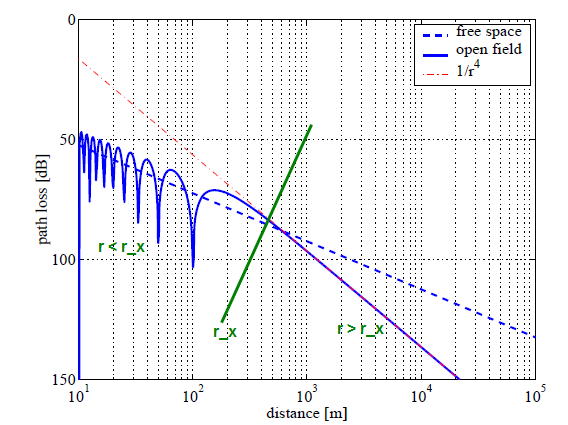
\includegraphics[width=8cm]{./bilder/propagation-simulation.png}
    } \\
\hline
\hline 
\parbox{10cm}{
    \textbf{Beugung (Diffraction) \formelbuch{158}}:\\
    \begin{liste}
        \item Weitere Verluste durch Beugung
        \item Beugungsparameter: $v=h\sqrt{\dfrac{2(d_1+d_2)}{\lambda d_1d_2}}$
        \item Zusätzlicher (zum Modell dazu) Pfadverlust: \\
        $L \approx 20\log (\sqrt 2\pi v) \approx 20\log \frac v{0.225} \quad
        v>1$
    \end{liste}
    \center{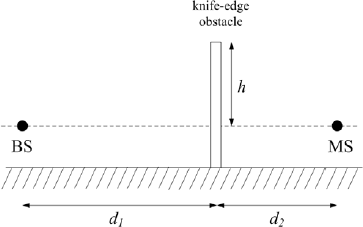
\includegraphics[width=5cm]{./bilder/propagation-diffraction.png}}
    }
    & \parbox{7cm}{
    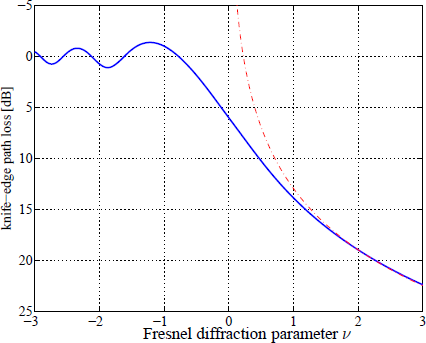
\includegraphics[width=7cm]{./bilder/propagation-fresnel-diffraction-parameter.png} } \\
\hline
\parbox{10cm}{
    \textbf{Fresnel-Zonen \formelbuch{163}}:\\
    \begin{liste}
        \item Keine Hindernisse innerhalb von gewissen ``Fresnel''-Zonen
        \item Fresnel-Zonen approximiert durch Radius: $r_n \approx
        \sqrt{\dfrac{n\lambda d_1 d_2}{d_1+d_2}}$
        \item Verbindung zum Fresnel-Parameter: $v=\frac h{r_1} \sqrt 2$
    \end{liste}
    }
    & \parbox{6cm}{
    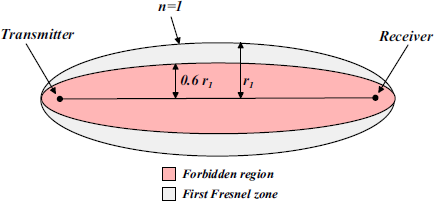
\includegraphics[width=6cm]{./bilder/propagation-fresnel-zones.png} } \\
\hline
\end{tabular}
\newpage
\begin{tabular}{ll}
\parbox{8cm}{   
    \subsection{Streuung (Scattering) \formelbuch{164}}
    \begin{liste}
        \item Entsteht, wenn Oberflächen rauh sind
        \item Keine Reflektionen in exakte Richtung
    \end{liste}
    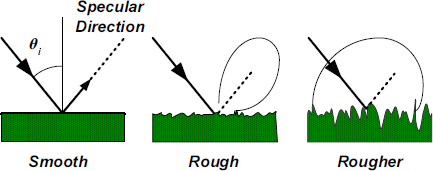
\includegraphics[width=6cm]{./bilder/propagation-scattering.png}}
& \parbox{10cm}{
    \subsection{Wetterabhängikeit \formelbuch{165}}
    \scriptsize
    \begin{tabular}{|l|r|r|r|r|r|} \hline
    \multicolumn{2}{|c|}{rain}&
    \multicolumn{4}{|c|}{frequency} \\ \hline
    type        & intensity  & 450\,MHz & 1\,GHz   &  3\,GHz  &  10\,GHz\\ 
    \hline\hline
    mizzle (drizzle)      & 0.25\,mm/h  & $2.2\cdot 10^{-8}$ & $1.5\cdot 10^{-6}$ & $1.5\cdot 10^{-4}$ & 0.02    \\ \hline
    light rain  &    5\,mm/h  & $1.0\cdot 10^{-6}$ & $2.0\cdot 10^{-5}$ & $1.0\cdot 10^{-3}$ & 0.08    \\ \hline
    medium rain & 12.5\,mm/h  & $3.0\cdot 10^{-6}$ & $7.0\cdot 10^{-5}$ & $3.0\cdot 10^{-3}$ & 0.28    \\ \hline
    heavy rain  &   25\,mm/h  & $7.5\cdot 10^{-6}$ & $1.5\cdot 10^{-4}$ & $1.0\cdot 10^{-2}$ & 0.6     \\ \hline
    shower      &   50\,mm/h  & $1.0\cdot 10^{-5}$ & $3.0\cdot 10^{-4}$ & $2.0\cdot 10^{-2}$ & 1.5     \\ \hline
    \end{tabular}
}
\end{tabular}


\begin{tabular}{ll}
\parbox{11cm}{
	\subsection{Link Budget \formelbuch{166}}
	\begin{liste}
	    \item Summierung aller (logarithmischen) Verluste und Gewinne vom Sender
	    zum Empfänger
	    \item Noise power density (Rauschleistung) $N_0 = -174\text{dBm}$ (pro Hz)
	    \item Empfänger- \& Sendergewinn ($G_T, G_R$) in DBi
	    \item Bsp: $P=N_0+10 \logd B+\text{NF}+\text{SNR}+L-G_T-G_R$
	\end{liste}

	\subsection{Fading \formelbuch{166}}
	\begin{liste}
	    \item Large Scale Fading
	    	\begin{liste}
	    		\item Auf Grund von Shadowing
	    		\item Log-Normal Fading
	    	\end{liste}
	    \item Small Scale Fading 
	    	\begin{liste}
		    	\item Reflexionen nahe Rx/Tx
		    	\item Rayleigh Fading
	    	\end{liste}
	\end{liste}
    }
& \parbox{7cm}{
    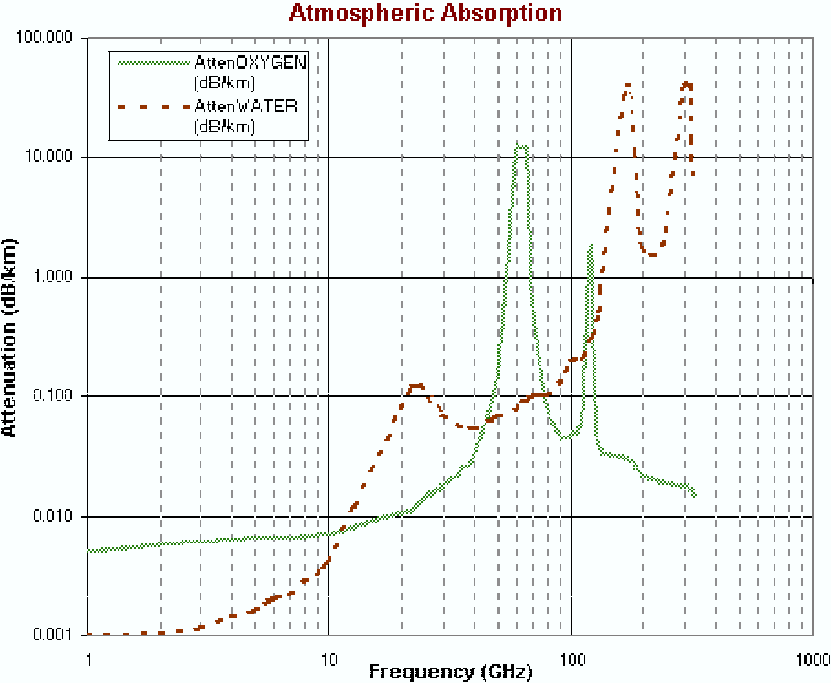
\includegraphics[width=7cm]{./bilder/propagation-atmospheric-absorption.png}}
\end{tabular}
\\
Klassifikation Small Scale Fading:\\
    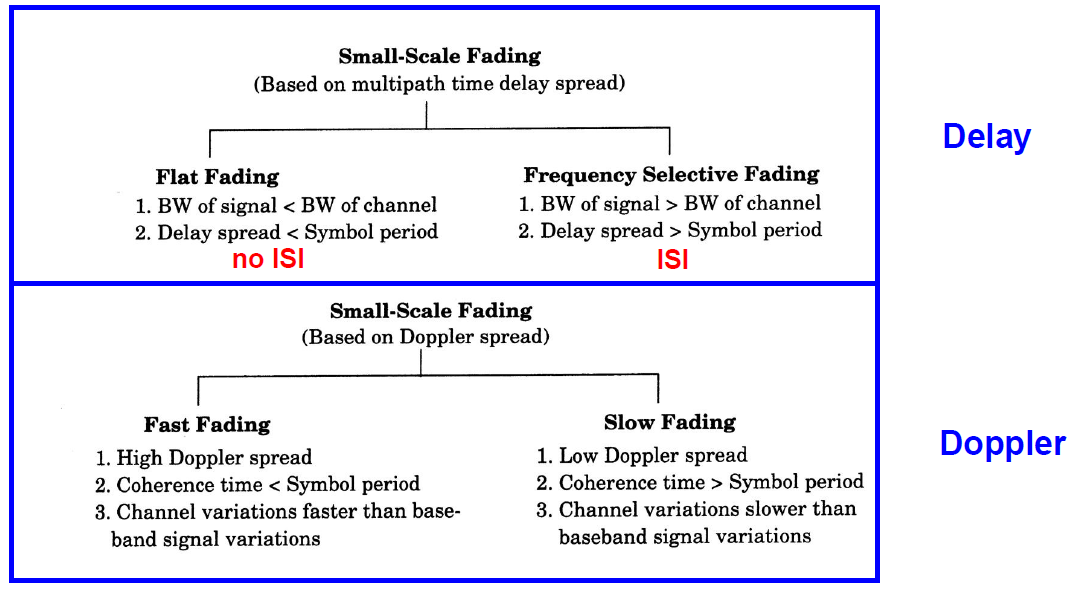
\includegraphics[width=7cm]{./bilder/classificationSmallScaleFading.png}
\subsection{Fast Fading \formelbuch{167}}
\begin{tabular}{|lll|}
\hline
\parbox{7cm}{
    \textbf{Non-line-of-sight (NLOS)} \\
    \begin{liste}
        \item Gehört zu flat fading (frequency non-selective)
        \item Rayleigh Verteilung $p(r) = \frac r{\sigma^2}
        e^{-\frac{r^2}{2\sigma^2}}$
    \end{liste}
    }
    & \parbox{5cm}{
        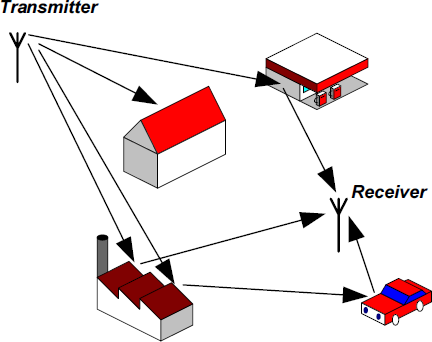
\includegraphics[width=5cm]{./bilder/propagation-nlos.png}
        } 
    &
    \multirow{2}{*}{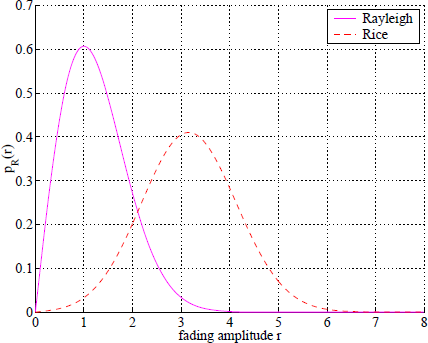
\includegraphics[width=5.5cm]{./bilder/propagation-fading-pdf.png}}
    \\
\parbox{7cm}{
    \textbf{Line-of-sight (LOS)} \\
    \begin{liste}
        \item Gehört zu flat fading (frequency non-selective)
        \item Rayleigh Verteilung $p(r) = \frac r{\sigma^2}
        e^{-\frac{r^2}{2\sigma^2}}$
    \end{liste}
    }
    & \parbox{5cm}{
        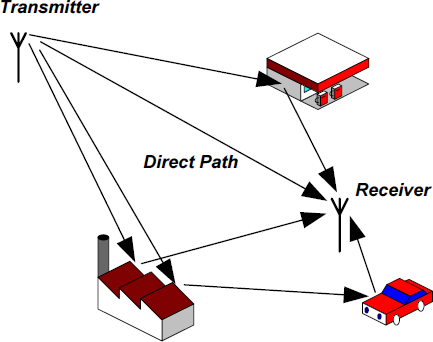
\includegraphics[width=5cm]{./bilder/propagation-los.png}
        } 
    & \\
\hline
\parbox{7cm}{
	    \textbf{Frequency selective fading (multipath)}
	    \begin{liste}
            \item {\em Mean delay}: $\tau_0=\frac 1{P_T}\sum\limits_k P_k
            \tau_k$
            \item {\em RMS delay spread}:\\
            $\tau_{\text{RMS}}=\sqrt{\frac{1}{P_T}}\sum\limits_k P_k
            (\tau_k-\tau_0)^2$
            \item Total power:
            $P_T=\sum\limits_k P_k$
        \end{liste}
    } 
    & \parbox{5cm}{
        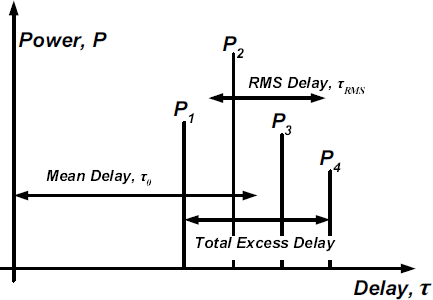
\includegraphics[width=5cm]{./bilder/propagation-frequency-selective-power-delay.png} 
        } 
    & \parbox{5cm}{ 
        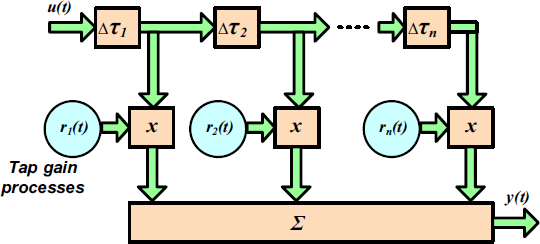
\includegraphics[width=5.5cm]{./bilder/propagation-frequency-selective-model.png} 
        } \\
\hline
\end{tabular}

\subsection{Beziehungen zwischen Fading Parameter \formelbuch{173}}
\begin{liste}
    \item $T_c \propto  \frac 1{f_m}$ \qquad $T_c$ = Kohärenzzeit, $f_m$ =
    Dopplerverschiebung (spread)
    \item $B_c \propto \frac 1{\tau}$ \qquad $B_c$ = Kohärenzbandbreite, $\tau$
    = Zeitverbreiterung (broadeing)
    \item $B_c$, $T_c$ unabhängig
\end{liste}
